% Autor: Manuel Lippert
% Physikalisches Praktikum

% Main-Datei für die Auswertung in TeX

% Struktur:
% Jedes Kapitel hat einen Input-File. Um Merge-Konflikte zu verhindern wird angeraten für jede 
% Datei eine eigene Tex Datei zu machen und sie im jeweiligen Kapitel zu importieren. Die in
% Input-Struktur dient zur besseren Übersicht und für mögliche Ordner, welche hier vorhanden sind. Die Zahlen vor den 
% Ordner dient zur Ordnung der einzelnen tex-Files nach Kapiteln


% Packages
\documentclass[paper=a4,bibliography=totoc,BCOR=10mm,numbers=noenddot,fontsize=11pt,headsepline]{scrreprt}              
                 
\usepackage[ngerman]{babel}
\usepackage[T1]{fontenc}
\usepackage[latin1, utf8]{inputenc} %ä, ö, ü inbegriffen
\usepackage[babel,german=quotes]{csquotes} %For Quotes
\usepackage{lmodern}
\usepackage{graphicx}
\usepackage{nicefrac}
\usepackage{fancyvrb}
\usepackage{amsmath,amssymb,amstext}
\usepackage{siunitx}
\usepackage{url}
\usepackage[numbers]{natbib}
\usepackage{microtype}
\usepackage[format=plain]{caption}
\usepackage{physics}
\usepackage{titleref} 

% Zusätzliche Packages
\usepackage{geometry} % Verändert Seitengeometrie
\usepackage{anyfontsize} % Alle Schriftgrößen möglich machen
\usepackage[table]{xcolor} % Farbliche Gestaltung Tabellen
\usepackage{ifthen} % Für kompliziertere tex-Files
\usepackage[absolute,overlay]{textpos} %Textboxen
\usepackage{amsfonts} % Schriftarten
\usepackage{xstring} % Stringoperationen
\usepackage{tikz} % Zeichnungen
\usepackage{pdfpages} % Import von pdfs (Protokolle)
\usepackage{hyperref} % Verlinkungen im Dokument
\usepackage{makecell}
\usepackage{subcaption}

% Abschnittseinrückung und -abstand
% Die folgenden Zeilen sollen möglichst nicht verändert werden
\parindent 0.0cm
\parskip 0.8ex plus 0.5ex minus 0.5ex

% Anzahl und Größe von Gleitobjekten
% maximal 2 Objekte oben und unten
% erlaubt auch größere Bilder, welche die ganze Seite benötigen
% Die folgenden Zeilen sollen möglichst nicht verändert werden
\setcounter{bottomnumber}{2}
\setcounter{topnumber}{2}
\renewcommand{\bottomfraction}{1.}
\renewcommand{\topfraction}{1.}
\renewcommand{\textfraction}{0.}

%\sc und \bc veraltet. Daher: (20.09.2018)
\DeclareOldFontCommand{\sc}{\normalfont\scshape}{\@nomath\sc}
\DeclareOldFontCommand{\bf}{\normalfont\scshape}{\textbf}

% Verschiedenes
\pagestyle{headings}          % Der Seitenstil sollte möglichst nicht verändert werden
\graphicspath{{./Bilder/}}    % Der Pfad für die Abbildungen Abbildungen wird gesetzt
\VerbatimFootnotes            % \verb etc. auch in \footnotes mφglich

% Funktionen
\newcommand\tab[1][1cm]{\hspace*{#1}}
\newcommand{\vect}[1]{\boldsymbol{\mathbf{#1}}}
\newcolumntype{g}{>{\columncolor[rgb]{ .741,  .843,  .933}}l}
% Tiefgestellte Zahlen nicht kursiv
\catcode`_=\active
\newcommand_[1]{\ensuremath{\sb{\mathrm{#1}}}}

\begin{document}

    \nonfrenchspacing

    % 0. Kapitel Cover
    % 0. Cover

% Hier sind nur die Variablen und der Abschnitt Informationen (unten) zu bearbeiten der REst läuft automatisch ab (z.b Farbenänderung)

% Noch abänderbar nur ein Vorschlag
\newgeometry{top=30mm, bottom=20mm, inner=20mm, outer=20mm}
\thispagestyle{empty}

% Colors (Notability Colors)
\definecolor{Notablue}{HTML}{3498DB}		
\definecolor{Notared}{HTML}{CF366C}			
\definecolor{Notagreen}{HTML}{19B092}		
\definecolor{Notaorange}{HTML}{FA9D00}		
\definecolor{Notagrey}{HTML}{969696}		
\definecolor{Notalavendel}{HTML}{9DBBD8}	

% Boolean by default false. Für Absatz in der Überschrift
\newboolean{twoRows}
\newboolean{symbol}

% Funktions
\makeatletter
   \def\vhrulefill#1{\leavevmode\leaders\hrule\@height#1\hfill \kern\z@}
\makeatother
\newcommand*\ruleline[1]{\par\noindent\raisebox{.8ex}{\makebox[\linewidth]{\vhrulefill{\linethickness}\hspace{1ex}\raisebox{-.8ex}{#1}\hspace{1ex}\vhrulefill{\linethickness}}}}

% Variables
\def\schriftgrosse{70}
\def\linethickness{1,5pt}

\def\farbe{black}
\def\fach{PPBphys2}
\def\name{Manuel Lippert - Paul Schwanitz}
\def\titel{Rasterelektronen- \\[0,5cm] mikroskop} % Absatz mit \\[0,5cm]; u = Übung, k = Klausur; s = Skript, e = Ergebnis
\def\bottom{WS2021/22}
\def\datum{13.09.2021}
\def\platz{NWII | 2.1.00.267}
\def\betreuer{Inga Elvers}

\def\teilnehmerm{Manuel Lippert}
\def\emailm{Manuel.Lippert@uni-bayreuth.de}
\def\teilnehmerp{Paul Schwanitz}
\def\emailp{Paul.Schwanitz@uni-bayreuth.de}

%\def\auswertp{}
%\def\messp{}
%\def\protop{}

\def\groupnr{11}

\begin{titlepage}
			
	\centering
	{\LARGE \sffamily {\textbf{\bottom}\par}}
	\vspace{2,5cm}
    {\fontsize{30}{0}\sffamily\ruleline{\textcolor{\farbe}{\textbf{\fach}}}\par}
    \vspace{6cm}
	{\Large\sffamily \ruleline{\name}\par}
		
	\IfSubStr {\titel} {\\[0,5cm]} {\setboolean{twoRows}{true}} {\setboolean{twoRows}{false}}
	
	\ifthenelse{\boolean{twoRows}}
		{
			\begin{textblock*}{21cm}(0cm,8cm) % {block width} (coords), centered		
				{\fontsize{\schriftgrosse}{0}\sffamily\textcolor{\farbe}{\textbf{\titel}}\par}
			\end{textblock*}
		}
		{
			\begin{textblock*}{21cm}(0cm,9cm) % {block width} (coords), centered		
				{\fontsize{\schriftgrosse}{0}\sffamily\textcolor{\farbe}{\textbf{\titel}}\par}
			\end{textblock*} 
		}
	
	% Choose Logo
	\ifthenelse {\equal{\farbe}{Notared}} {\def\logo{Bilder/Logo/UniBTNotared}}
		{\ifthenelse {\equal{\farbe}{Notagreen}} {\def\logo{Bilder/Logo/UniBTNotagreen}}
			{\ifthenelse {\equal{\farbe}{Notablue}} {\def\logo{Bilder/Logo/UniBTNotablue}}
				{\ifthenelse {\equal{\farbe}{Notaorange}} {\def\logo{Bilder/Logo/UniBTNotaorange}}
					{\ifthenelse {\equal{\farbe}{Notagrey}} {\def\logo{Bilder/Logo/UniBTNotagrey}}
						{\ifthenelse {\equal{\farbe}{Notalavendel}} {\def\logo{Bilder/Logo/UniBTNotalavendel}}	
							{\ifthenelse {\equal{\farbe}{black}} {\def\logo{Bilder/Logo/UniBT}}	
								{\def\logo{noLogo}}
							}
						}
					}
				}
			}
		}	

	\IfSubStr{\logo}{noLogo}{\setboolean{symbol}{false}}{\setboolean{symbol}{true}}
	
	% Gruppe
	\vspace{10cm}
	{\large\sffamily{Gruppe \groupnr}}
	
	%Logo
	\vfill

	\ifthenelse{\boolean{symbol}}
		{
			\begin{figure}[h]
			\begin{center}
				
				\includegraphics[width=2cm]{\logo}
				
			\end{center}
			\end{figure}
		}
	
\end{titlepage}

\restoregeometry

% Information
\chapter*{Informationen}
\label{chap:info}

\begin{tabular}{l l}

	{\textbf{Versuchstag}} \hspace{1cm} & \hspace{1cm} {\datum}\\[0,2cm]
	{\textbf{Versuchsplatz}} \hspace{1cm} & \hspace{1cm} {\platz}\\[0,2cm]
	{\textbf{Betreuer}} \hspace{1cm} & \hspace{1cm} {\betreuer}\\[1,2cm]
	{\textbf{Gruppen Nr.}} \hspace{1cm} & \hspace{1cm} {\groupnr}\\[0.2cm]
	% Für Fortgeschittenenen Praktikum
	{\textbf{Teilnehmer}} \hspace{1cm} & \hspace{1cm} {\teilnehmerm~(\emailm)}\\[0.2cm]
						  \hspace{1cm} & \hspace{1cm} {\teilnehmerp~(\emailp)}\\[0.2cm]
	% Für Grundpraktikum
	%{\textbf{Auswertperson}} \hspace{1cm} & \hspace{1cm} {\auswertp}\\[0.2cm]
	%{\textbf{Messperson}} \hspace{1cm} & \hspace{1cm} {\messp}\\[0.2cm]
	%{\textbf{Protokollperson}} \hspace{1cm} & \hspace{1cm} {\protop}\\[0.2cm]

\end{tabular}

    \thispagestyle{empty}
    \cleardoublepage
    \tableofcontents
    \cleardoublepage

    % 1. Kapitel Einleitung
    % 1. Einleitung

\chapter{Einleitung}
\label{chap:einleitung}

Durch elektronische Messung ist jede Messung eines Signals einem gewissen Anteil von Rauschen behaftet. Um die Messung so präzise wie möglich durchführen zu können muss man zu den Mitteln der Signal/Rausch-Verbesserung greifen. Dafür ist wichtig die jeweiligen Störquellen zu identifizieren und diese bestenfalls zu eliminieren oder in praktischsten Fall zu unterdrücken.\\

In diesem Versuch werden die Methoden und die auswirkung der Signal/Rausch-Verbesserung diskutiert. Dabei werden unterschiedliche zeitliche Signalformen mit überlagertem Rau-
schen über die „Fast Fourier Transformationsmethode“ (FFT) und der Mittlung der Signal diskutiert. Zudem werden die grundlegenden Arten von elektronischen Filter und deren Effekt in der Praxis angewendet und analysiert. Auch das Lock-In Verfahren wird Anhand eines Lock-In Verstärkers näher betrachtet.

    % 2.Kapitel Theorie
    \chapter{Theoretical background}

\section{Saturation spectroscopy in general}
With saturation spectroscopy enables us to see the hyperfine structure, because with this methode it is theoretical possible to bypass the dopplereffect. \\
By saturation spectroscopy a laser (pump beam) beam will pass a gas sample (with doppler widened absorption transitions). That caused a stimulation of specific atoms, depending from there speed. 

Vice versa to the pump beam another laser beam with the same frequency (probe beam) will also pass the gas sample.

If now a photon is absorbed, the atom must have a speed component ($v_z$ parallel to the laser beams) in the intervall: 
\begin{align}
    v_{\text{z}} \pm \Delta v_{\text{z}} = \frac{\omega -\omega_0 \pm \delta \omega_{\text{n}}}{k}
\end{align}
In this connection: 
\begin{itemize} 
    \item $\delta \omega_{\text{n}}$ is the homogeneous line width.
    \item $\Delta v_{\text{z}}$ is the width of the hole in the occupation distribution.
    \item $\omega$ is the frequency of the laser.
    \item $\omega_0$ is the resonance frequency of the wanted transition.
    \item $k$ 
\end{itemize}

Because many atoms are stimulated, the probe beam hits barley atoms that can be stimulated. For this reason we obtain the occupation distribution $N(v_{\text{z}})$ and the adsorption profile $\alpha(\omega)$. For this experiment the laser frequency is so chosen, that the fit with the resonance frequency of the wanted transition \citep{VA}.

\section{Preparatory questions}

\paragraph{1. Nuclear spin}
Because the isotopes have a different nuclear structure and the spin depends on that structure, the spins are different. Below the quantum numbers of the basic condition and the fist two stimulated conditions: 
\begin{table}[h]
    \centering
    \begin{tabular}{|c|c|c|c|c|}
        \hline
        Element Name & basic condition & first stimulated condition & second stimulated condition \\
        \hline\hline
        Rb-85 & $5^2$S$_{\frac{1}{2}}$ $\Rightarrow$ F = 2, 3 & $5^2$P$_{\frac{1}{2}}$ $\Rightarrow$ F = 2, 3 & $5^2$S$_{\frac{3}{2}}$ $\Rightarrow$ F = 1, 2, 3, 4 \\
        \hline
        Rb-87 & $5^2$S$_{\frac{1}{2}}$ $\Rightarrow$ F = 1, 2 & $5^2$P$_{\frac{1}{2}}$ $\Rightarrow$ F = 1, 2 & $5^2$S$_{\frac{3}{2}}$ $\Rightarrow$ F = 0, 1, 2, 3 \\
        \hline
    \end{tabular}
    \caption{Quantum numbers of Rb-85 and Rb-87}
\end{table}

\newpage
\paragraph{2. Importent terms}

\subparagraph{Natural line width}

\subparagraph{Doppler broadening}

\subparagraph{Homogeneous/inhomogeneous widening}

\subparagraph{Saturation widening}


\paragraph{3. Cross-over resonances}


\paragraph{4. Beam splitter and $\lambda$/2 plate}


\paragraph{5. Hyperfine structure}

    % 3.Kapitel Protokoll
    % Charlotte Geiger - Manuel Lippert - Leonard Schatt
% Physikalisches Praktikum

% 3.Kapitel  Protokoll

% Variables
\def\skalierung{0.65}

\chapter{Messprotokoll}
\label{chap:protokoll}

Das Messprotokoll wurde am Versuchstag handschriftlich erstellt und hier als
PDF-Datei eingefügt. Dabei wurden Durchführung und Aufbau schon vorher in dieses
Dokument beschrieben, je nachdem. test

%\centering

% Einbindung des Protokolls als pdf (mit Seitenzahl etc.)
% Erste Seite mit Überschrift
%\includepdf[pages = 1, landscape = false, nup = 1x1, scale = \skalierung , pagecommand={\thispagestyle{empty}\chapter{Protokoll}}]
%            {03 Protokoll/Protokoll.pdf}
% Restliche Seiten richtig skaliert
\includepdf[pages = 2-, landscape = false, nup = 1x1, scale = \skalierung , pagecommand={}]
            {03-Protokoll/ProtokollSP.pdf}

    % 4.Kapitel Versuchsauswertung
    % 4. Versuchsauswertung

\chapter{Auswertung und Diskussion}
\label{chap:versuchsauswertung}

% Text

% Input der Teilauswertung je nach Produktion der Nebendateien ohne Ordner
% Teilauswertung X

\section{Teilauswertung X}
% Teilauswertung 4
\section{Lebenszeitmessung}
\label{sec:lebenszeit}

CFP1-c1 5.008 2.9295095907141993 \\
CFP2-c1 5.008 2.86328777266995 \\
CFP3-c1 5.008 2.864972335683961 \\
YFP1-c2 5.008 3.25925836091248 \\
YFP2-c2 5.008 3.4119299746334164 \\
YFP3-c2 5.008 3.3295197646160584 \\

% etc.

    % 5.Kapitel Fazit
    % Charlotte Geiger - Manuel Lippert - Leonard Schatt
% Physikalisches Praktikum

% 5. Kapitel Einleitung

\chapter{Fazit}
\label{chap:fazit}

% Platz für Text

    % Anhang
    \chapter{Peaks für den Depolarisationsgrad}
\begin{figure}[h]
  \centering
  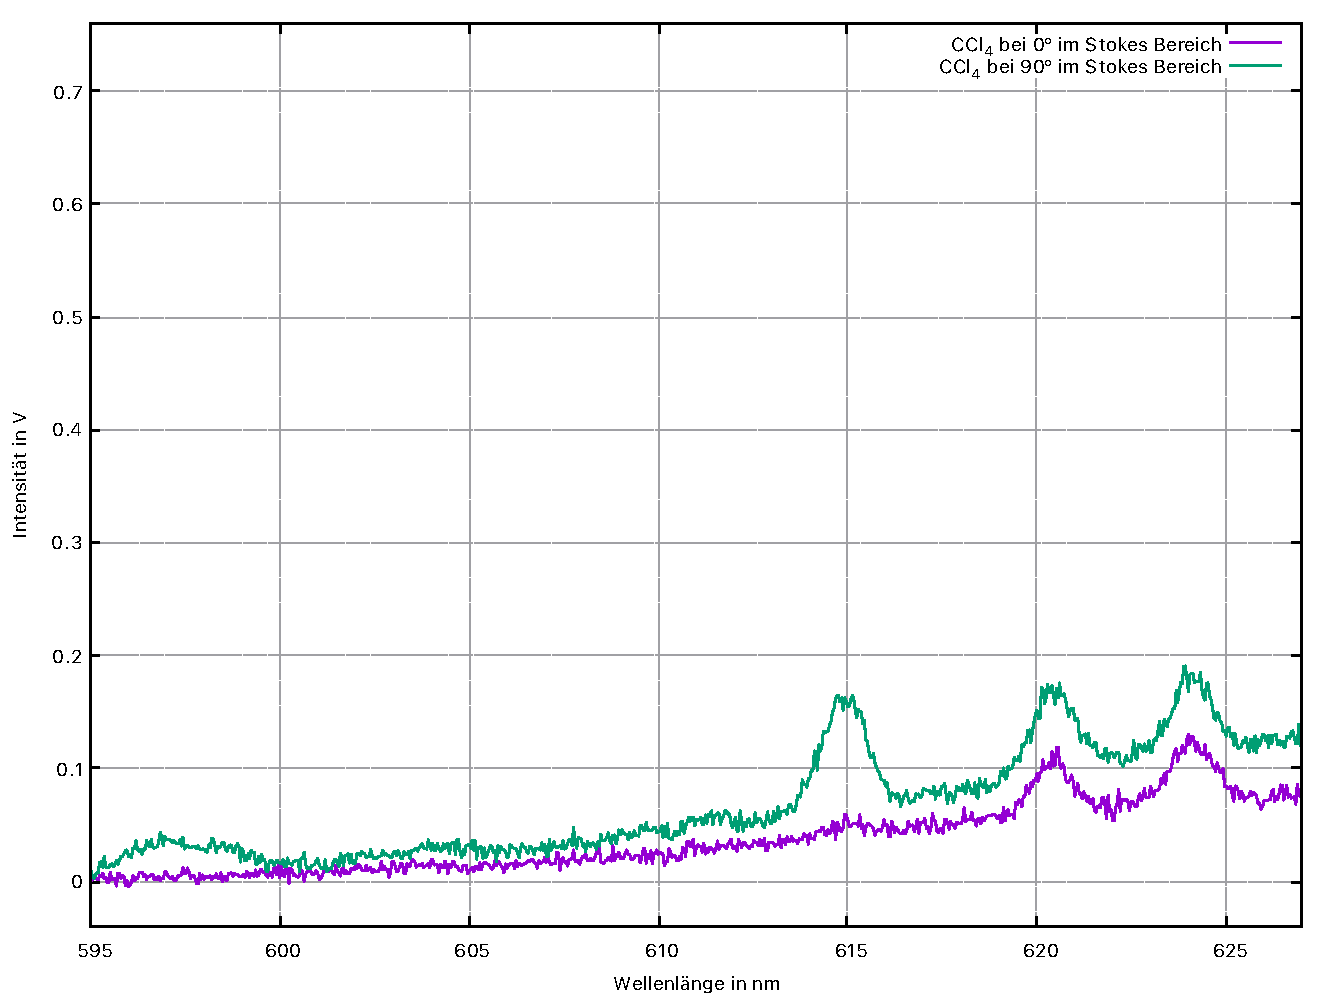
\includegraphics[scale=0.45]{Bilder/Verbesserung_Auswertung/ccl4_stokes.pdf}
  \caption{Spektrum von $CCl_4$, im Stokes Bereich bei 0° und 90° Polarisation.}
\end{figure}
\begin{figure}[h]
  \centering
  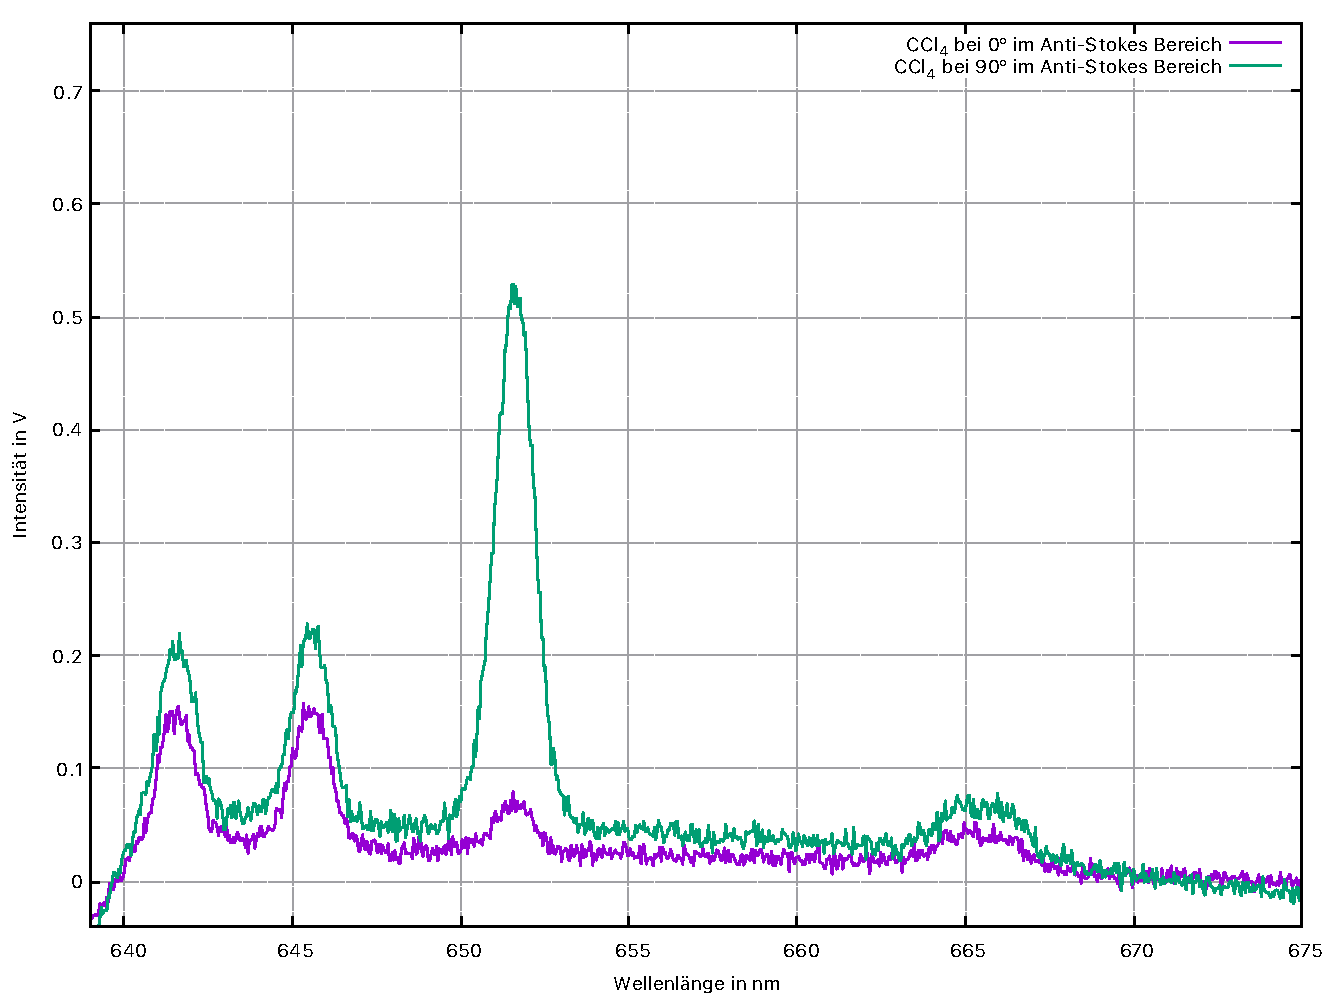
\includegraphics[scale=0.45]{Bilder/Verbesserung_Auswertung/ccl4_anti.pdf}
  \caption{Spektrum von $CCl_4$, im Anti-Stokes Bereich bei 0° und 90° Polarisation.}
\end{figure}
\begin{figure}[h]
  \centering
  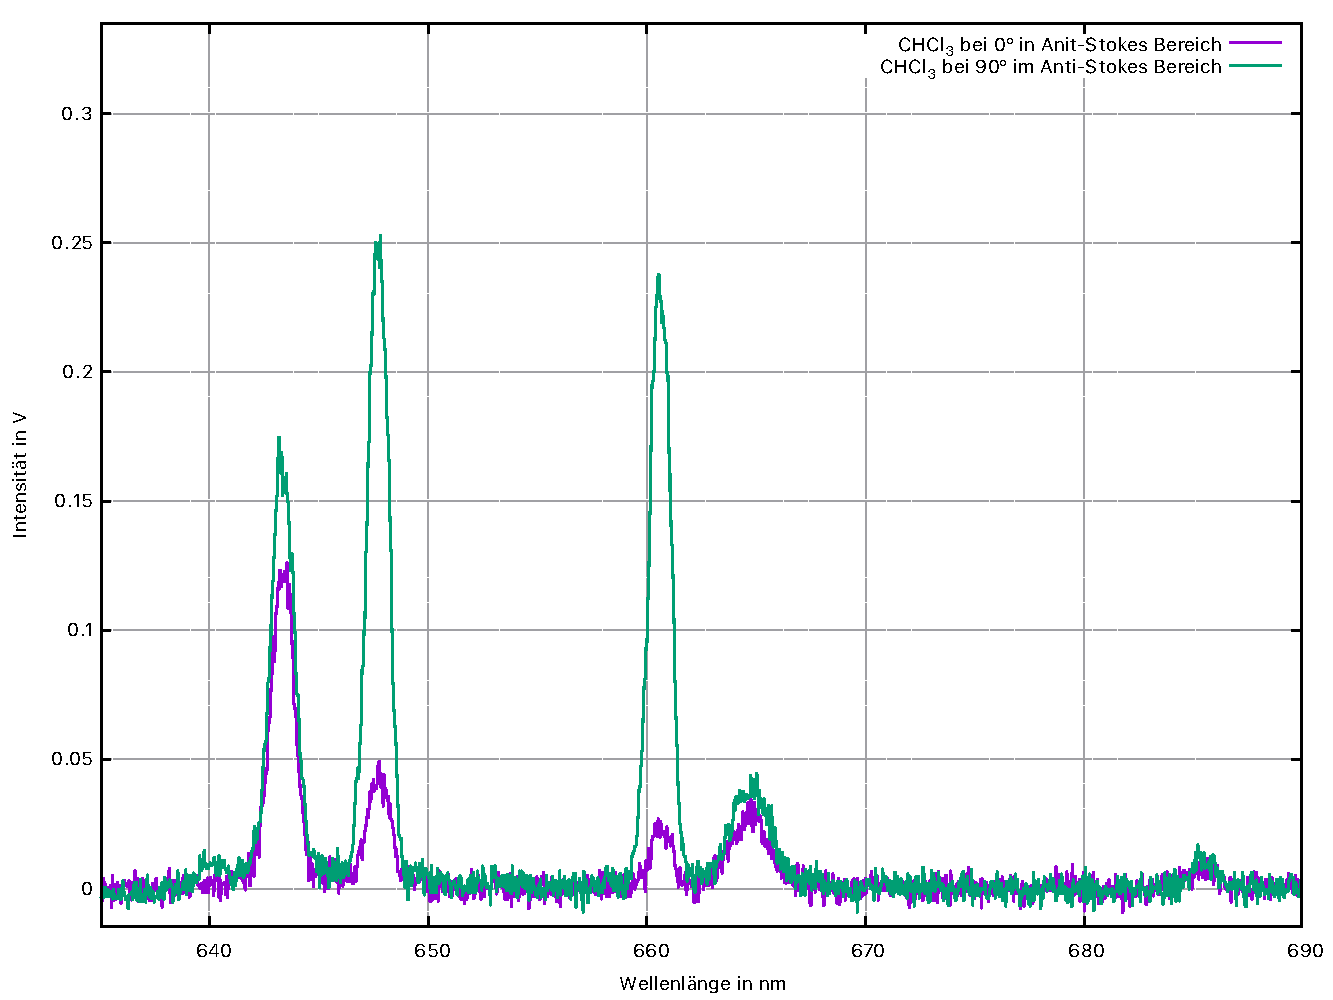
\includegraphics[scale=0.5]{Bilder/Verbesserung_Auswertung/chcl3_anti.pdf}
  \caption{Spektrum von $CHCl_3$, im Anti-Stokes Bereich bei 0° und 90° Polarisation.}
\end{figure}
\begin{figure}[h]
  \centering
  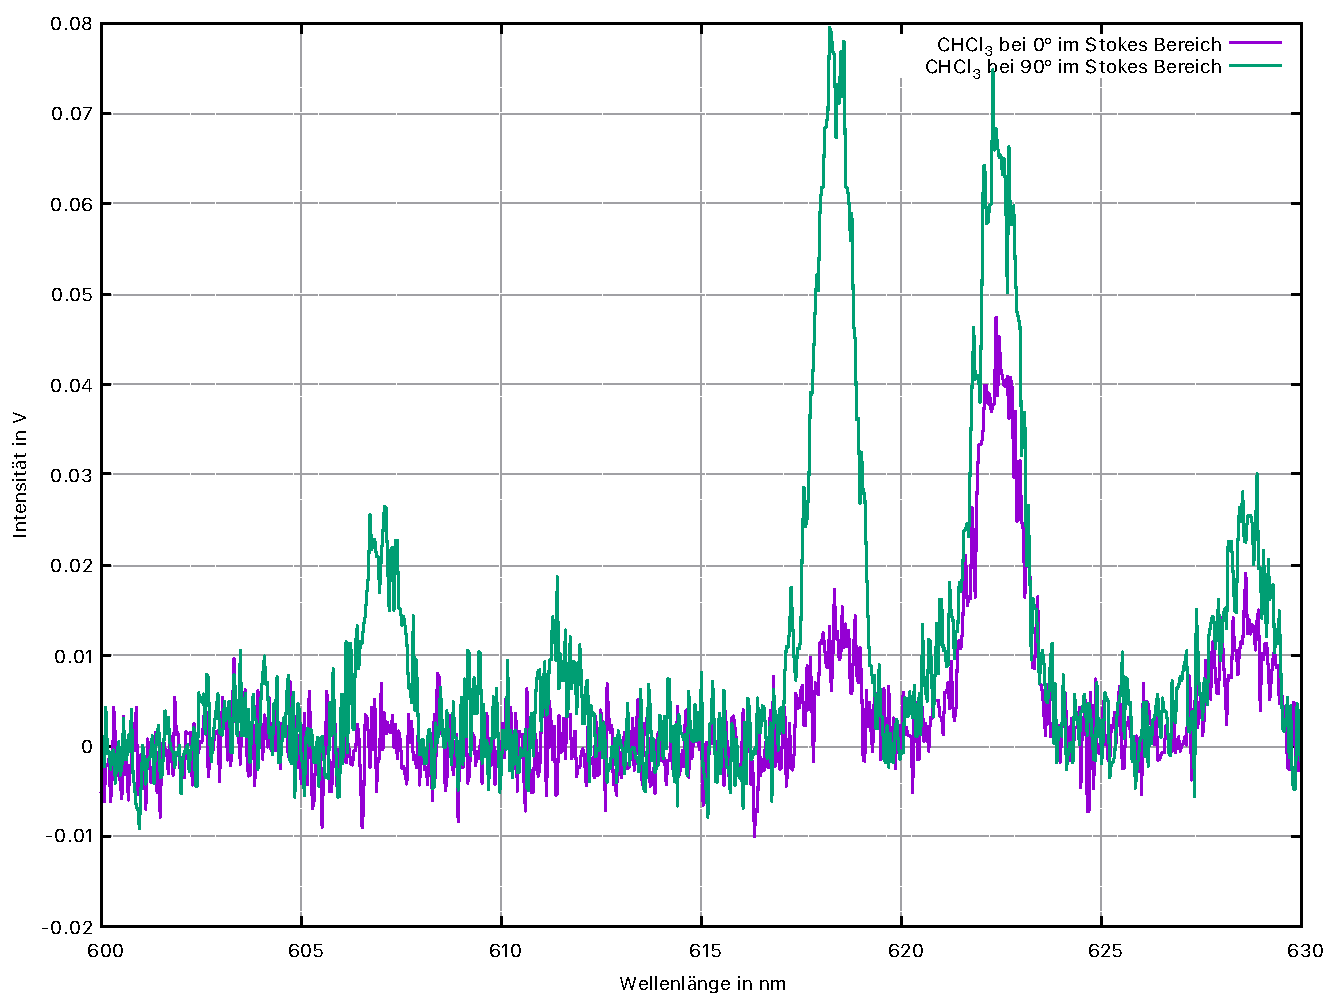
\includegraphics[scale=0.5]{Bilder/Verbesserung_Auswertung/chcl3_stokes.pdf}
  \caption{Spektrum von $CHCl_3$, im Stokes Bereich bei 0° und 90° Polarisation. In dem Bereich, indem es zur Überschneidung in der Wellenlänge bei den Peaks sowohl bei 0° als auch bei 90° kommt.}
\end{figure}

\chapter{Werte für Lage der Raman-Linien}
\begin{table}[h]
    \centering
    \begin{tabular}{c||c|c|c|c|c|c|c}
      \makecell{ $\lambda$ \\in nm} & $\nu$ in $\frac{1}{\text{cm}}$  & \makecell{ Fehler \\ $s_{\nu}$ in $\frac{1}{\text{cm}}$} & \makecell{Intensität\\ $0^{\circ}$ in V}  &  \makecell{Intensität\\ $90^{\circ}$ in V}  & \makecell{ Depolarisations- \\ grad $\rho$}  & \makecell{ Fehler \\ Depol. $s_{\rho}$} & Polarisation \\
      \hline
      643,3 & 270,4 & 12,1  & 0,1210 & 0,1688 & 0,7171 & 0,0365 & Depol. \\
      647,7 & 376,0 & 11,9  & 0,0470 & 0,2499 & 0,1879 & 0,0204 & Pol. \\
      660,7 & 679,8 & 11,5  & 0,0218 & 0,2279 & 0,0958 & 0,0220 & Pol. \\
      664,9 & 775,4 & 11,3  & 0,0281 & 0,0346 & 0,8123 & 0,1861 & Depol. \\
      685,3 & 1223,1 & 10,7  & 0,0088 & 0,0138 & 0,6359 & 0,4287 & Depol. \\  
    \end{tabular}
    \caption{Wellenlänge, Wellenzahl, Fehler der Wellenzahl, Intensität für 90° und 0°, Depolarisationsgrad und Fehler des Depolarisationsgrad für $CHCl_3$ im Anti-Stokes-Bereich.}
\end{table}
\begin{table}[h]
    \centering
    \begin{tabular}{c||c|c|c|c|c|c|c}
      \makecell{ $\lambda$ \\in nm} & $\nu$ in $\frac{1}{\text{cm}}$  & \makecell{ Fehler \\ $s_{\nu}$ in $\frac{1}{\text{cm}}$} & \makecell{Intensität\\ $0^{\circ}$ in V}  &  \makecell{Intensität\\ $90^{\circ}$ in V}  & \makecell{ Depolarisations- \\ grad $\rho$}  & \makecell{ Fehler \\ Depol. $s_{\rho}$} & Polarisation \\
    \hline
    643,3 & 270,4 & 12,1  & 0,1059 & 0,1747 & 0,6063 & 0,0335 & Depol. \\
    647,7 & 376,0 & 11,9  & 0,0434 & 0,2581 & 0,1681 & 0,0196 & Pol. \\
    659,9 & 661,5 & 11,5  & 0,0274 & 0,2651 & 0,1033 & 0,0190 & Pol. \\
    663,7 & 748,2 & 11,4  & 0,0320 & 0,0474 & 0,6754 & 0,1272 & Depol. \\
    671,4 & 921,0 & 11,1  & 0,0092 & 0,0181 & 0,5082 & 0,3092 & Depol. \\
  \end{tabular}%
\caption{Wellenlänge, Wellenzahl, Fehler der Wellenzahl, Intensität für 90° und 0°, Depolarisationsgrad und Fehler des Depolarisationsgrad für $CDCl_3$ im Anti-Stokes-Bereich.}
\end{table}\newpage
\begin{table}[h]
    \centering
    \begin{tabular}{c||c|c|c|c|c|c|c}
      \makecell{ $\lambda$ \\in nm} & $\nu$ in $\frac{1}{\text{cm}}$  & \makecell{ Fehler \\ $s_{\nu}$ in $\frac{1}{\text{cm}}$} & \makecell{Intensität\\ $0^{\circ}$ in V}  &  \makecell{Intensität\\ $90^{\circ}$ in V}  & \makecell{ Depolarisations- \\ grad $\rho$}  & \makecell{ Fehler \\ Depol. $s_{\rho}$} & Polarisation \\
      \hline
      639,0 & 165,8 & 12,3  & 0,0345 & 0,0655 & 0,5274 & 0,0863 & Depol. \\
      641,7 & 231,7 & 12,2  & 0,1201 & 0,7271 & 0,1652 & 0,0070 & Pol. \\
      655,1 & 550,4 & 11,7  & 0,0409 & 0,3626 & 0,1127 & 0,0139 & Pol. \\
      660,1 & 666,1 & 11,5  & 0,0841 & 0,1200 & 0,7007 & 0,0509 & Depol. \\  
    \end{tabular}%
    \caption{Wellenlänge, Wellenzahl, Fehler der Wellenzahl, Intensität für 90° und 0°, Depolarisationsgrad und Fehler des Depolarisationsgrad für $CHBr_3$ im Anti-Stokes-Bereich.}
\end{table}%
\begin{table}[h]
    \centering
    \begin{tabular}{c||c|c|c|c|c|c|c}
      \makecell{ $\lambda$ \\in nm} & $\nu$ in $\frac{1}{\text{cm}}$  & \makecell{ Fehler \\ $s_{\nu}$ in $\frac{1}{\text{cm}}$} & \makecell{Intensität\\ $0^{\circ}$ in V}  &  \makecell{Intensität\\ $90^{\circ}$ in V}  & \makecell{ Depolarisations- \\ grad $\rho$}  & \makecell{ Fehler \\ Depol. $s_{\rho}$} & Polarisation \\
      \hline
      641,5 & 226,8 & 12,2  & 0,1437 & 0,2009 & 0,7151 & 0,0306 & Depol. \\
      645,7 & 328,2 & 12,0  & 0,1472 & 0,2257 & 0,6520 & 0,0264 & Depol. \\
      651,7 & 470,8 & 11,8  & 0,0707 & 0,5163 & 0,1370 & 0,0098 & Pol. \\
      665,5 & 789,0 & 11,3  & 0,0381 & 0,0658 & 0,5793 & 0,0878 & Depol. \\  
    \end{tabular}
    \caption{Wellenlänge, Wellenzahl, Fehler der Wellenzahl, Intensität für 90° und 0°, Depolarisationsgrad und Fehler des Depolarisationsgrad für $CCl_4$ im Anti-Stokes-Bereich.}
  \end{table}%

    % Literatur
    \bibliographystyle{plainnat}
    \bibliography{Auswertung.bib}

\end{document}